%%% main.tex %%%

%%%%% --------------------------------------------- %%%%%
%	 				  PRÁCTICAS DE						%
%		  TECNOLOGÍAS DE DESARROLLO DE SOFTWARE         %
%														%
%                  JOSÉ SALINAS PARDO                   %
%                 HUGO SÁNCHEZ MARTÍNEZ                 %
%%%%% --------------------------------------------- %%%%%

\documentclass[11pt]{article}
%%% style.tex %%%

%%%%% --------------------------------------------- %%%%%
%	   PACKAGES AND OTHER DOCUMENT CONFIGURATIONS       %
%%%%% --------------------------------------------- %%%%%


\usepackage{amsmath,amsfonts,stmaryrd,amssymb} % Math packages
\usepackage{fancyhdr}
\usepackage{enumerate} % Custom item numbers for enumerations
\usepackage[ruled]{algorithm2e} % Algorithms
\usepackage[framemethod=tikz]{mdframed} % Custom boxed/framed environments

\definecolor{codegray}{gray}{0.925}
\let\colortexttt\texttt
\renewcommand{\texttt}[1]{\colorbox{codegray}{\colortexttt{#1}}}

\usepackage{xcolor} % Colours
\definecolor{mRed}{rgb}{0.8, 0, 0}
\definecolor{mGreen}{rgb}{0,0.6,0}
\definecolor{mGray}{rgb}{0.5,0.5,0.5}
\definecolor{mPurple}{rgb}{0.58,0,0.82}
\definecolor{backgroundColour}{rgb}{0.95,0.95,0.92}

\usepackage{listings} % File listings, with syntax highlighting
\lstset{
	basicstyle=\ttfamily, % Typeset listings in monospace font
	extendedchars=true,  % Soporta caracteres extendidos
	literate={├}{{|-}}1 {─}{{-}}1 {●}{{$\bullet$}}1 {└}{{\texttt{\textbackslash}}}1
}
\lstdefinestyle{PythonStyle}{
	backgroundcolor=\color{backgroundColour},   
	commentstyle=\color{mGreen}\textit,
	keywordstyle=\color{magenta}\bfseries,
	numberstyle=\tiny\color{mGray},
	stringstyle=\color{mPurple},
	basicstyle=\fontfamily{pcr}\selectfont\footnotesize,
	breakatwhitespace=false,         
	breaklines=true,
	captionpos=b,                    
	keepspaces=true,                 
	numbers=left,                    
	numbersep=5pt,
	showspaces=false,                
	showstringspaces=false,
	showtabs=false,                  
	tabsize=2,
	language=Python,
	extendedchars=true,
	inputencoding=utf8
}

\lstdefinestyle{BashStyle}{
	backgroundcolor=\color{lightgray!10},
	keywordstyle=\color{blue!80!black}\bfseries,
	stringstyle=\color{red!70!black},         
	basicstyle=\fontfamily{pcr}\selectfont\small,
	breakatwhitespace=false,
	breaklines=true,
	captionpos=b,
	keepspaces=true,
	numbers=none,                  
	showspaces=false,
	showstringspaces=false,
	showtabs=false,
	tabsize=2,
	language=bash,
	extendedchars=true,
	inputencoding=utf8
}

\lstdefinestyle{TextFileStyle}{
	backgroundcolor=\color{lightgray!5},
	basicstyle=\ttfamily\small,
	numbers=none,
	breaklines=true,
	captionpos=b,
	frame=single,
	rulecolor=\color{gray!30},
	showstringspaces=false,
	tabsize=2,
	language={}
}

\usepackage{colortbl} % Para \arrayrulecolor y colorear tablas
\usepackage{alltt}
\usepackage{array, multirow, tabularx, booktabs} % Tables
\usepackage{float}
\usepackage{tikz}
\usetikzlibrary{quotes,babel, positioning, shapes, shapes.geometric, arrows, calc, external, chains, shadows}
% \usetikzlibrary{arrows.meta, positioning, chains, positioning, shapes.geometric, shadows}
\usepackage{aeguill}
\usepackage{tikzpeople}

\usepackage{pgfplots}

\usepackage[linktoc=none]{hyperref} % para enlaces. linktoc deshabilita indice
\hypersetup{
	colorlinks,
	linkcolor={red}, % footnotes
	urlcolor={blue!80!black}, % urls
	pdftitle={Documentación AppChat},
	pdfsubject={TDS},
	pdfauthor={José Salinas Pardo, Hugo Sánchez Martínez}
}

\usepackage[spanish, es-nodecimaldot]{babel} % Paquete de español

\setlength{\arrayrulewidth}{1.5\arrayrulewidth} % Table rule thickness

% Cambiar título del ToC
\addto\captionsspanish{
	\renewcommand{\contentsname}
	{Contenidos}%
}

\usepackage{listingsutf8}    % Soporte para caracteres UTF-8
\usetikzlibrary{shadows,calc}

\usepackage[inline]{enumitem}   
\makeatletter
% This command ignores the optional argument for itemize and enumerate lists
\newcommand{\inlineitem}[1][]{%
	\ifnum\enit@type=\tw@
	{\descriptionlabel{#1}}
	\hspace{\labelsep}%
	\else
	\ifnum\enit@type=\z@
	\refstepcounter{\@listctr}\fi
	\quad\@itemlabel\hspace{\labelsep}%
	\fi}
\makeatother
\parindent=0pt

% some parameters for customization
\def\shadowshift{3pt,-3pt}
\def\shadowradius{6pt}

\colorlet{innercolor}{black!50}
\colorlet{outercolor}{gray!05}

% this draws a shadow under a rectangle node
\newcommand\drawshadow[1]{
	\begin{pgfonlayer}{shadow}
		\shade[outercolor,inner color=innercolor,outer color=outercolor] ($(#1.south west)+(\shadowshift)+(\shadowradius/2,\shadowradius/2)$) circle (\shadowradius);
		\shade[outercolor,inner color=innercolor,outer color=outercolor] ($(#1.north west)+(\shadowshift)+(\shadowradius/2,-\shadowradius/2)$) circle (\shadowradius);
		\shade[outercolor,inner color=innercolor,outer color=outercolor] ($(#1.south east)+(\shadowshift)+(-\shadowradius/2,\shadowradius/2)$) circle (\shadowradius);
		\shade[outercolor,inner color=innercolor,outer color=outercolor] ($(#1.north east)+(\shadowshift)+(-\shadowradius/2,-\shadowradius/2)$) circle (\shadowradius);
		\shade[top color=innercolor,bottom color=outercolor] ($(#1.south west)+(\shadowshift)+(\shadowradius/2,-\shadowradius/2)$) rectangle ($(#1.south east)+(\shadowshift)+(-\shadowradius/2,\shadowradius/2)$);
		\shade[left color=innercolor,right color=outercolor] ($(#1.south east)+(\shadowshift)+(-\shadowradius/2,\shadowradius/2)$) rectangle ($(#1.north east)+(\shadowshift)+(\shadowradius/2,-\shadowradius/2)$);
		\shade[bottom color=innercolor,top color=outercolor] ($(#1.north west)+(\shadowshift)+(\shadowradius/2,-\shadowradius/2)$) rectangle ($(#1.north east)+(\shadowshift)+(-\shadowradius/2,\shadowradius/2)$);
		\shade[outercolor,right color=innercolor,left color=outercolor] ($(#1.south west)+(\shadowshift)+(-\shadowradius/2,\shadowradius/2)$) rectangle ($(#1.north west)+(\shadowshift)+(\shadowradius/2,-\shadowradius/2)$);
		\filldraw ($(#1.south west)+(\shadowshift)+(\shadowradius/2,\shadowradius/2)$) rectangle ($(#1.north east)+(\shadowshift)-(\shadowradius/2,\shadowradius/2)$);
	\end{pgfonlayer}
}

% create a shadow layer, so that we don't need to worry about overdrawing other things
\pgfdeclarelayer{shadow} 
\pgfsetlayers{shadow,main}

\newsavebox\mybox
\newlength\mylen

\newcommand\shadowimage[2][]{%
	\setbox0=\hbox{\includegraphics[#1]{#2}}
	\setlength\mylen{\wd0}
	\ifnum\mylen<\ht0
	\setlength\mylen{\ht0}
	\fi
	\divide \mylen by 120
	\def\shadowshift{\mylen,-\mylen}
	\def\shadowradius{\the\dimexpr\mylen+\mylen+\mylen\relax}
	\begin{tikzpicture}
		\node[anchor=south west,inner sep=0] (image) at (0,0) {\includegraphics[#1]{#2}};
		\drawshadow{image}
\end{tikzpicture}}

\renewcommand{\footnoterule}{%
	\vspace{1cm} % Espacio adicional antes de la línea
	\hrule width 0.8\textwidth % Ajusta el ancho de la línea (80% del ancho del texto)
	\vspace{2cm} % Espacio adicional después de la línea
}


%%%%% --------------------------------------------- %%%%%
%	                 DOCUMENT MARGINS
%%%%% --------------------------------------------- %%%%%

\usepackage{geometry} % Required for adjusting page dimensions and margins

\geometry{
	a4paper, % Papaer size
	margin={2cm,3cm},
	headheight=14pt, % Header height
	footskip=1cm, % Space from the bottom margin to the baseline of the footer
	headsep=1.2cm, % Space from the top margin to the baseline of the header
	%showframe, % Uncomment to show how the type block is set on the page
}

%%%%% --------------------------------------------- %%%%%
%	                      FONTS                         %
%%%%% --------------------------------------------- %%%%%

\usepackage[utf8]{inputenc} % Required for inputting international characters
\usepackage[T1]{fontenc} % Output font encoding for international characters
\usepackage[
protrusion=true,
activate={true,nocompatibility},
final,
tracking=true,
kerning=true,
spacing=true,
factor=1100]{microtype}
\SetTracking{encoding={*}, shape=sc}{40}


% Choose font:
\usepackage{mathptmx} 	 % Times
% \usepackage{mathpazo}  % Palatino
% \usepackage{lmodern}	 % Upgraded LaTeX font

%%%%% --------------------------------------------- %%%%%
%	            COMMAND LINE ENVIRONMENT                %
%%%%% --------------------------------------------- %%%%%

% Usage:
% \begin{commandline}
	%	\begin{verbatim}
		%		$ ls
		%		
		%		Applications	Desktop	...
		%	\end{verbatim}
	% \end{commandline}

\mdfdefinestyle{commandline}{
	leftmargin=10pt,
	rightmargin=10pt,
	innerleftmargin=15pt,
	middlelinecolor=black!50!white,
	middlelinewidth=2pt,
	frametitlerule=false,
	backgroundcolor=black!5!white,
	frametitle={Bash},
	frametitlefont={\normalfont\sffamily\color{white}\hspace{-1em}},
	frametitlebackgroundcolor=black!50!white,
	nobreak,
}

% Define a custom environment for command-line snapshots
\newenvironment{commandline}{
	\medskip
	\begin{mdframed}[style=commandline]
	}{
	\end{mdframed}
	\medskip
}

%%%%% --------------------------------------------- %%%%%
%	             FILE CONTENTS ENVIRONMENT              %
%%%%% --------------------------------------------- %%%%%

% Usage:
% \begin{file}[optional filename, defaults to "File"]
	%	File contents, for example, with a listings environment
	% \end{file}

\mdfdefinestyle{file}{
	innertopmargin=1.6\baselineskip,
	innerbottommargin=0.8\baselineskip,
	innerleftmargin=1.6\baselineskip,
	topline=false, bottomline=false,
	leftline=false, rightline=false,
	leftmargin=2cm,
	rightmargin=2cm,
	singleextra={%
		\draw[fill=black!10!white](P)++(0,-1.2em)rectangle(P-|O);
		\node[anchor=north west]
		at(P-|O){\ttfamily\mdfilename};
		%
		\def\l{3em}
		\draw(O-|P)++(-\l,0)--++(\l,\l)--(P)--(P-|O)--(O)--cycle;
		\draw(O-|P)++(-\l,0)--++(0,\l)--++(\l,0);
	},
	nobreak,
}

% Define a custom environment for file contents
\newenvironment{file}[1][File]{ % Set the default filename to "File"
	\medskip
	\newcommand{\mdfilename}{#1}
	\begin{mdframed}[style=file]
	}{
	\end{mdframed}
	\medskip
}

%%%%% --------------------------------------------- %%%%%
%	          NUMBERED QUESTIONS ENVIRONMENT            %
%%%%% --------------------------------------------- %%%%%

% Usage:
% \begin{question}[optional title]
	%	Question contents
	% \end{question}

\mdfdefinestyle{question}{
	innertopmargin=1.2\baselineskip,
	innerbottommargin=0.8\baselineskip,
	roundcorner=5pt,
	nobreak,
	singleextra={%
		\draw(P-|O)node[xshift=1em,anchor=west,fill=white,draw,rounded corners=5pt]{%
			Question \theQuestion\questionTitle};
	},
}

\newcounter{Question} % Stores the current question number that gets iterated with each new question

% Define a custom environment for numbered questions
\newenvironment{question}[1][\unskip]{
	\bigskip
	\stepcounter{Question}
	\newcommand{\questionTitle}{~#1}
	\begin{mdframed}[style=question]
	}{
	\end{mdframed}
	\medskip
}


%%%%% --------------------------------------------- %%%%%
%	              WARNING TEXT ENVIRONMENT              %
%%%%% --------------------------------------------- %%%%%

% Usage:
% \begin{warn}[optional title, defaults to "Warning:"]
	%	Contents
	% \end{warn}

\mdfdefinestyle{warning}{
	topline=false, bottomline=false,
	leftline=false, rightline=false,
	nobreak,
	singleextra={%
		\draw(P-|O)++(-0.5em,0)node(tmp1){};
		\draw(P-|O)++(0.5em,0)node(tmp2){};
		\fill[black,rotate around={45:(P-|O)}](tmp1)rectangle(tmp2);
		\node at(P-|O){\color{white}\scriptsize\bf !};
		\draw[very thick](P-|O)++(0,-1em)--(O);%--(O-|P);
	}
}

% Define a custom environment for warning text
\newenvironment{warn}[1][Warning:]{ % Set the default warning to "Warning:"
	\medskip
	\begin{mdframed}[style=warning]
		\noindent{\textbf{#1}}
	}{
	\end{mdframed}
}


%%%%% --------------------------------------------- %%%%%
%                 INFORMATION ENVIRONMENT               %
%%%%% --------------------------------------------- %%%%%

% Usage:
% \begin{info}[optional title, defaults to "Info:"]
	% 	contents
	% 	\end{info}

\mdfdefinestyle{info}{%
	topline=false, bottomline=false,
	leftline=false, rightline=false,
	nobreak,
	singleextra={%
		\fill[black](P-|O)circle[radius=0.4em];
		\node at(P-|O){\color{white}\scriptsize\bf i};
		\draw[very thick](P-|O)++(0,-0.8em)--(O);%--(O-|P);
	}
}

% Define a custom environment for information
\newenvironment{info}[1][Info:]{ % Set the default title to "Info:"
	\medskip
	\begin{mdframed}[style=info]
		\noindent{\textbf{#1}}
	}{
	\end{mdframed}
}



\begin{document}

\title{
	\vspace{-5ex}
	\begin{figure}[H]
		\centering
		
\includegraphics[width=72mm]{umu-logo}
	\end{figure}
	
	{\Large \textsc{Universidad de Murcia}}\\
	{\Large Facultad de Informática}\\ [12.5ex]
	{\Large \textsc{Prácticas de}\\ [1ex]}
	{\Huge Tecnologías de Desarrollo de Software}\\ [1ex]
	{\Large \textsc{3º de Grado en Ingeniería Informática}}\\
	{\Large \textsc{Profesor: Fco. Javier Bermudez Ruiz}} \\
	{\Large \textsc{Grupo 2.3}} \\
	{\Large \textsc{Curso 2024/2025}} \\ 
	\vspace{10ex}
}

\author{
	{\Large José Salinas Pardo}\\[0.5ex]
	48740555J\\
	\texttt{j.salinaspardo@um.es}
	\and
	{\Large Hugo Sánchez Martínez}\\[0.5ex]
	24450997L\\
	\texttt{hugo.s.m@um.es}\\
}

\pagestyle{fancy}
\fancyhf{}
\fancyhead[LE]{\nouppercase{\rightmark} \hfill \textbf{\nouppercase{\leftmark}}}   % Encabezado en la página izquierda (even) sin mayúsculas
\fancyhead[RO]{\nouppercase{\rightmark}}  % Encabezado en la página derecha (odd) sin mayúsculas
\setlength{\headheight}{25pt}  % Ajusta la altura del encabezado
\fancyfoot[R]{J. Salinas, H. Sánchez}
\fancyfoot[C]{\thepage}

\date{\vspace{-10ex}}
\maketitle
\thispagestyle{empty} % Elimina el número de página de la portada
\clearpage

\thispagestyle{empty} % Elimina el número de página del ToC
\tableofcontents
\clearpage
\thispagestyle{empty} % Elimina el número de página del ToC
\listoffigures
\clearpage
\setcounter{page}{1}



\thispagestyle{empty}

\hrule
\vspace{-5.4ex}
\begin{abstract}
\vspace{1ex}
Este documento especifica la implementación de las prácticas de la asignatura Tecnologías de Desarrollo de Software del tercer curso del grado en Ingeniería Informática de la Universidad de Murcia.\\

Dicha práctica consiste en el desarrollo de una aplicación de mensajería (\textit{chatting}), \textbf{AppChat}, basada en aplicaciones ya existentes. El objetivo de este documento es describir en detalle el proceso de desarrollo de la aplicación, desde la planificación inicial y el análisis de requisitos, hasta la implementación y las pruebas finales.
\vspace{0.5ex}
\end{abstract}
\hrule
\vspace{4ex}

\section{Introducción}

\textbf{AppChat} es una aplicación de escritorio de mensajería instantánea desarrollada en Java 8. Basada en soluciones reales como \textit{Telegram} o \textit{Whatsapp}, AppChat permite a los usuarios llevar una gestión simple de sus contactos, ofreciendo la posibilidad de crear grupos y enviar mensajes como si fuesen ``\textit{grupos de difusión}''.\\

Además, AppChat implementa funcionalidad extra para sus miembros ``\textit{premium}''. Estos pueden exportar sus conversaciones con sus contactos de una forma sencilla gracias a la librería \textit{iText}.

\section{Requisitos}

AppChat requiere al menos tener instalada al menos la versión 8 de \href{https://www.oracle.com/java/technologies/javase/javase8-archive-downloads.html}{Java SE} para ejecutar.\\

Es necesario tener instalado Maven para poder gestionar las dependencias del proyecto correctamente.

\section{Tecnologías}

Durante el desarrollo de AppChat se han usado las siguientes tecnologías:

\begin{itemize}
	\item \textbf{Git}: Para el control de versiones y colaboración en el desarrollo.
	\item \textbf{Maven}: Utilizado como herramienta de gestión y construcción del proyecto.
	\item \textbf{Eclipse}: Se ha escodigo Eclipse como entorno de desarrollo (IDE).
	\item \textbf{PlantUML}: Usado para generar los diagramas UML del modelo.
	\item \textbf{Java Swing}: Biblioteca gráfica empleada para el desarrollo de la interfaz de usuario.
\end{itemize}

\clearpage

\section{Requisitos y Modelado de Clases}

\subsection{\textit{User Story Mapping}}

Realizamos una \textbf{representación visual} de las funcionalidades de la aplicación desde la perspectiva de usuario. El eje horizontal representa el flujo de trabajo de un usuario en un orden lógico, mientras que el eje vertical organiza las historias en función de su importancia.

\begin{figure}[h]
    \centering
    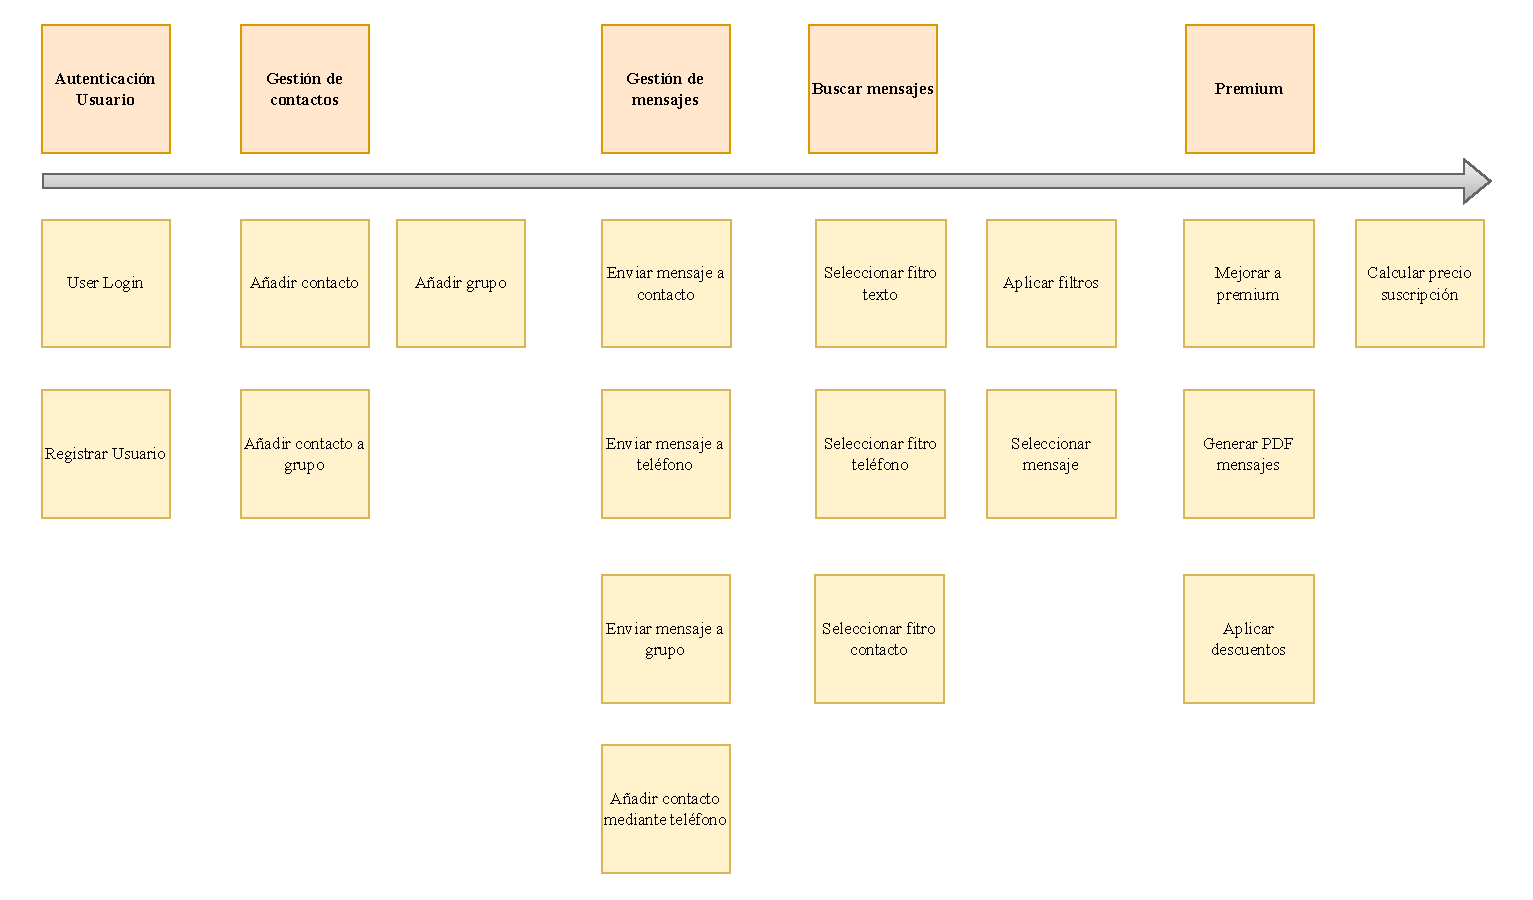
\includegraphics[width=0.8\linewidth]{figures/user-story-mapping.drawio-2.pdf}
    \caption{Diagrama de historias de usuario de AppChat}
    \label{fig:user-story-mapping}
\end{figure}

\subsection{Diagrama de secuencia: añadir miembro a grupo}

La funcionalidad tomada de ejemplo es la de crear un grupo, pero es válida ya que esta añade de forma secuencial varios miembros al grupo.

\begin{figure}[H]
	\centering
	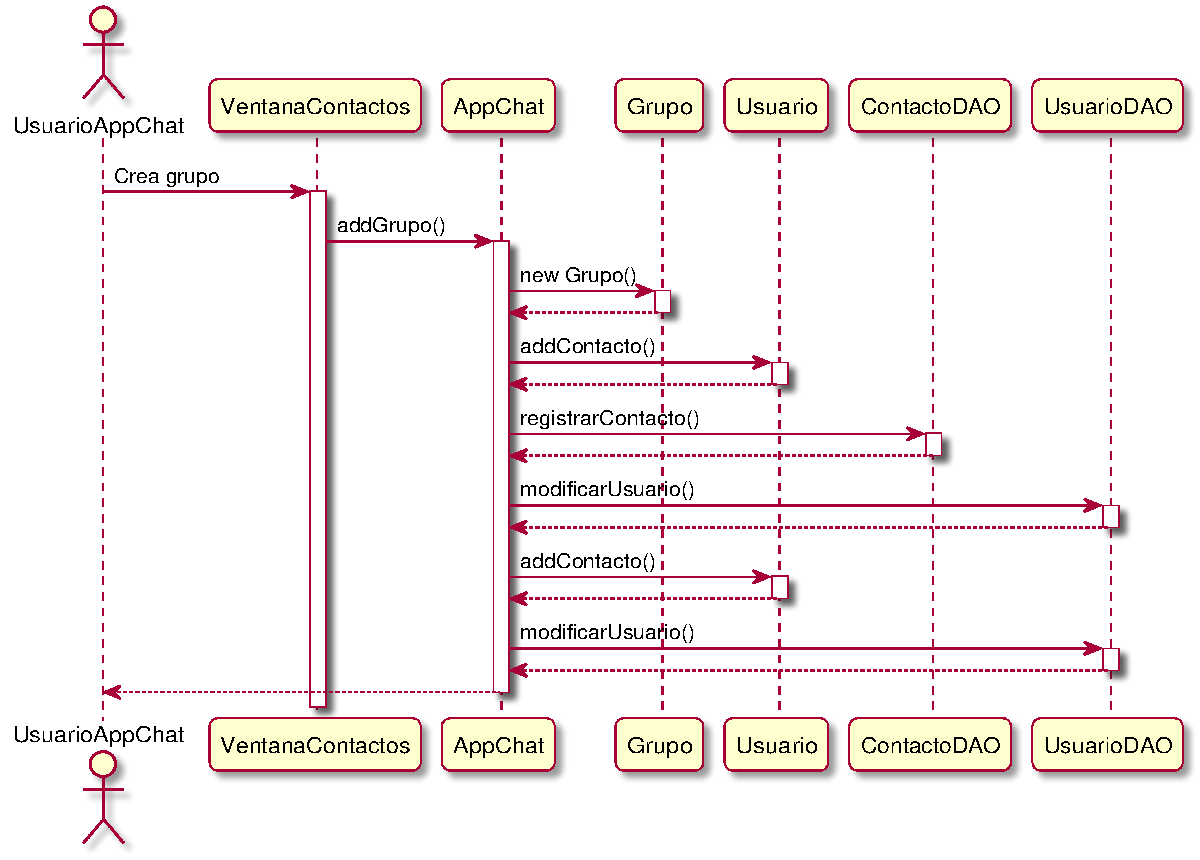
\includegraphics[width=0.5\linewidth]{figures/crear_grupo}
	\caption{Diagrama de secuencia simplificado para añadir miembro a grupo}
	\label{fig:crear-grupo}
\end{figure}

\subsection{Diagrama de clases}

\begin{figure}[H]
	\centering
	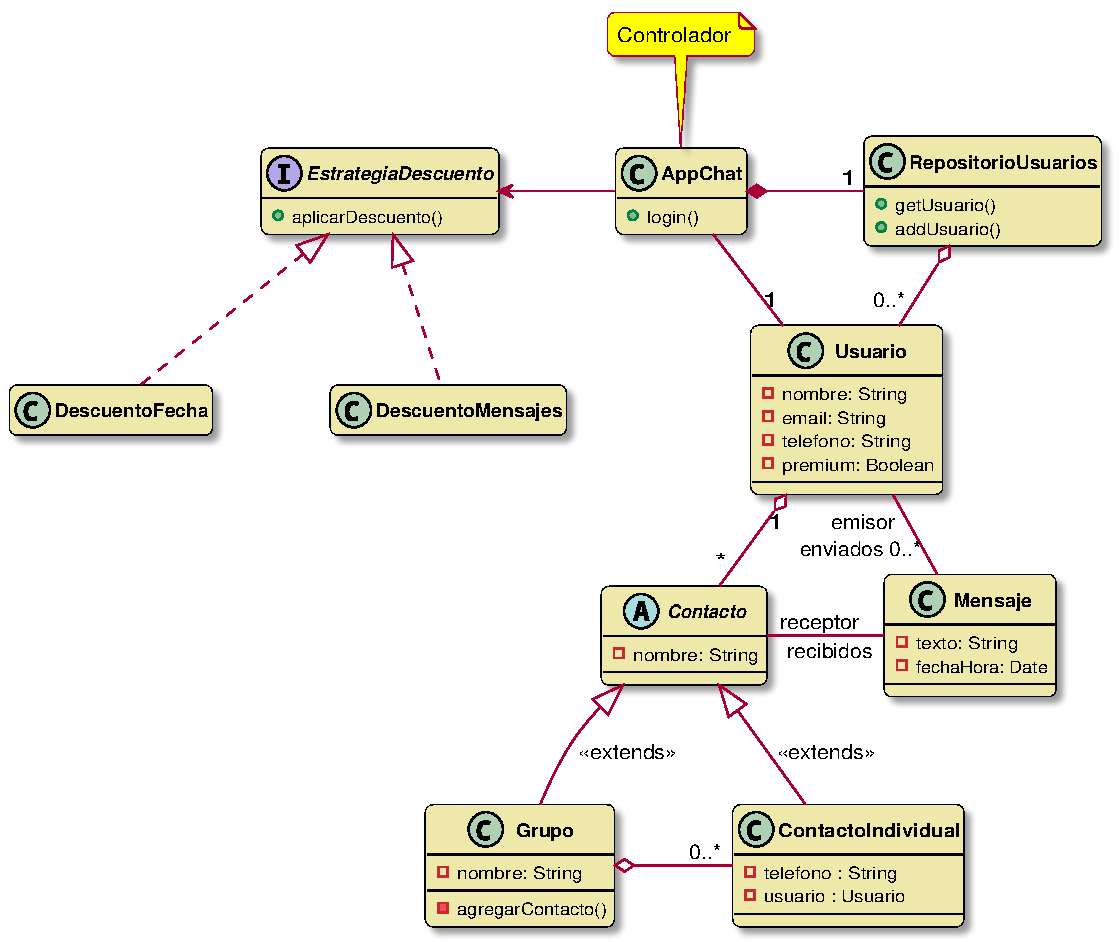
\includegraphics[width=0.7\linewidth]{figures/modelo}
	\caption{Modelo de clases de AppChat}
	\label{fig:modelo}
\end{figure}

Se ha optado por seguir la recomendación de los profesores de la asignatura, con ligeros cambios. La figura~\ref{fig:modelo} no muestra todos los atributos y métodos, solo los más relevantes.

\begin{itemize}
	\item \texttt{AppChat}: Siguiendo el principio MVC que se explicará más adelante, esta clase actúa de \guillemotleft \textit{controladora}\guillemotright \ de la aplicación.
	\item \texttt{RepositorioUsuarios}: Contiene una collección de los usuarios gestionados. Para la lógica de la aplicación, además de las entidades persistentes en la base de datos, es necesario llevar un control de todos los usuarios. Es invocada por el controlador con frecuencia, por ejemplo, para cargar los usuarios al iniciar la aplicación.
	\item \texttt{Usuario}: Representa al usuario de AppChat. Incluye operaciones para interactuar con sus contactos.
	\item \texttt{Contacto}: Clase abstracta que representa una forma de contacto con otro usuario. TODO.
	\begin{itemize}
		\item \texttt{ContactoIndividual}: Representa el contacto íntegro de la aplicación. Está asociado a un usuario de AppChat y tiene asignado un nombre de contacto.
		\item \texttt{Grupo}: Clase que modela un chat formado por un conjunto de contactos. Tiene un único administrador.
	\end{itemize}
	\item \texttt{Mensaje}: Clase que representa todo lo relacionado con un mensaje en la aplicación. Tiene como emisor un objeto \texttt{Usuario} y como receptor un objeto \texttt{Contacto}, que puede ser una persona o un grupo.
	\item \texttt{EstrategiaDescuento}: Interfaz necesaria para implementar diferentes descuentos usando el patrón de diseño ``\textit{strategy}''.
    \begin{itemize}
		\item \texttt{DescuentoFecha}: Estrategia de descuento que está disponible para el usuario si su fecha de nacimiento está entre un intervalo establecido por el sistema.
		\item \texttt{DescuentoMensajes}: Estrategia de descuento que aplica un porcentaje al precio base si el usuario supera un límite establecido de mensajes enviados en la aplicación.
	\end{itemize}
\end{itemize}

También se han diseñado otras clases como:

\begin{itemize}
	\item \texttt{App}: Lanzador de la aplicación.
	\item \texttt{CriteriosBusqueda}
	\item \texttt{BuscadosMensajes}
\end{itemize}

\clearpage

\section{Arquitectura de la aplicación}

\subsection{Patrón MVC}

AppChat sigue el patrón de arquitectura de software Modelo-Vista-Controlador. Este patrón nos permite separar los datos y la lógica del negocio de una aplicación de la interfaz que ve el usuario, conéctandolos a través de un controlador, permitiendo así tres componentes distintos:~\cite{mdnMVC}

\begin{itemize}
	\item \textbf{Vista (\textit{View}):} Representa la interfaz de usuario y todas las herramientas con las cuales el usuario hace uso del programa.
	
	\item \textbf{Modelo (\textit{Model}):} Es dónde está toda la lógica del negocio, la representación de todo el sistema, incluida la interacción con una base de datos, si es que el programa así lo requiere.
	
	\item \textbf{Controlador (\textit{Controller}):} Este componente es el que responde a la interacción (eventos) que realiza el usuario en la interfaz y realiza las peticiones al modelo para luego pasarlas a la vista. Aún no está del todo claro, pero con el siguiente ejemplo lo comprenderemos mejor.
\end{itemize}

\begin{figure}[H]
	\centering
	\scalebox{1.25}{
		\begin{tikzpicture}[
node distance = 3em and 3em,
start chain = going below,
    box/.style = {rectangle, rounded corners, draw=gray, thick,
        minimum height=2.5em, minimum width=10em, align=flush center,
        top color=#1!60, bottom color=#1!10,
        drop shadow, on chain},
    msg/.style={-latex, dashed},
    doublemsg/.style={latex-latex},
    msglabel/.style={above, yshift=-0.5em},
    database/.style={draw, cylinder, aspect=2, shape border rotate=90, minimum width=5em, minimum height=3em, on chain, cylinder uses custom fill, cylinder body fill=gray!10, cylinder end fill=gray!20},
]
                        
\node[businessman,label=Usuario, on chain] (Usr) {};
\node (V) [box=red]   {Vista};
\node (C) [box=blue]  {Controlador};
\node (M) [box=green] {Modelo};

\draw[doublemsg] (Usr) to node[msglabel, xshift=-2.25em] {\scriptsize Interactúa} (V);

\draw[msg] (V) to[bend right=40] node[msglabel, xshift=-2em] {\scriptsize Solicita} (C);
\draw[msg] (C) to[bend right=40] node[msglabel, xshift=2em] {\scriptsize Actualiza} (V);

\draw[msg] (C) to[bend right=40] node[msglabel, xshift=-2em] {\scriptsize Notifica} (M);
\draw[msg] (M) to[bend right=40] node[msglabel, xshift=2em] {\scriptsize Responde} (C);

\draw[doublemsg] (Usr) to node[above, xshift=-2.25em, yshift=-0.5em] {\scriptsize Interactúa} (V);

\node[database] (db) {} ;

\node[right=0.5em of db, yshift=0.5em] {\scriptsize Base de Datos H2};

\draw[doublemsg] (M) to node[above, xshift=-2.25em, yshift=-0.5em] {\scriptsize DAO} (db);

\end{tikzpicture}

	}
	\caption{Patrón de arquitectura software MVC}
	\label{fig:mvc}
\end{figure}

\clearpage

\subsection{Estructura general de la aplicación}

\begin{figure}[H]
	\centering
	\shadowimage[width=0.4\linewidth]{figures/hierarchy}
	\caption{Jerarquía de paquetes de AppChat}
	\label{fig:paquetes}
\end{figure}

La aplicación se estructura en 5 paquetes diferentes, cada uno con una funcionalidad específica. Cómo se ha comentado, los paquetes model, controlador y vista, forman parte del patrón MVC. Por su parte, 

\subsection{Decisiones de diseño relevantes}

\section{Patrones de diseño}

A lo largo del desarrollo de la aplicación, se han adoptado los principales patrones de diseño vistos en clase y se han implementado directamente en el código.

\subsection{Patrones creacionales}

Según \textit{Gamma et al}.~\cite{book:204958}\ el objetivo principal de los patrones de diseño creacionales es el de \textbf{abstraer el proceso de instanciación y creación de objetos}. Los patrones creacionales permiten además encapsulan el conocimiento sobre las clases concretas que utiliza el sistema, así como ocultar el proceso de creación y ensamblación de instancias por parte de las clases.

\subsubsection*{Singleton}

Utilizamos el patrón \textit{singleton} para aquellas clases de las que nos interesa tener una única instancia y permitir un acceso global a ella. En AppChat, siguen este patrón la clases controlador \texttt{AppChat}, el repositorio \texttt{RepositorioUsuarios}, la clase ``\textit{factoría}'' \texttt{DAOFactory} y el resto de clases ``\textit{adaptador}'' del paquete \texttt{umu.tds.dao.tds}.

\begin{figure}[H]
	\centering
	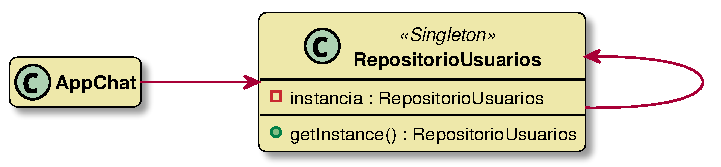
\includegraphics[width=0.6\linewidth]{figures/singleton_model}
	\caption{Modelo de \textit{Singleton} en AppChat}
	\label{fig:singleton}
\end{figure}

\subsubsection*{Factoría abstracta}

Este patrón se usa para las clases relacionadas con el ámbito de la persistencia en la aplicaicón. Se define una clase abstracta \texttt{DAOFactory} implementada como singleton y con métodos para obtener los distintos adaptadores disponibles. 

\subsection{Patrones estructurales}

\subsubsection*{Adaptador}

El patrón \textit{adapter} o adaptador permite que clases con interfaces incompatibles colaboren entre sí sin necesidad de modificar su código fuente. Usamos este patrón en las clases del paquete \texttt{umu.tds.dao.tds} para adaptar la funcionalidad de la clase \texttt{ServicioPersistencia} a las interfaces DAO definidas en \texttt{umu.tds.dao}. En la figura~\ref{fig:absfactory} se puede ver con más claridad la interrelación entre las clases.

\subsubsection*{Facade}

El patrón \textit{facade} o fachada se usa para proporcionan una interfaz que actúa como actúa como punto de acceso simplificado a un subsistema complejo. Su objetivo principal es ocultar la complejidad interna de varias clases colaboradoras y ofrecer una interfaz más clara y coherente.~\cite{refactoringGuruFacade}\\

Este patrón se usa en la clase controlador \texttt{AppChat}. Como se puede ver en el diagrama de sencuencia~\ref{fig:facade}, para operaciones como ``\textit{añadir contacto}'' es necesario una interfaz que oculte los complejas operaciones que conlleva la función.

\begin{figure}[H]
	\centering
	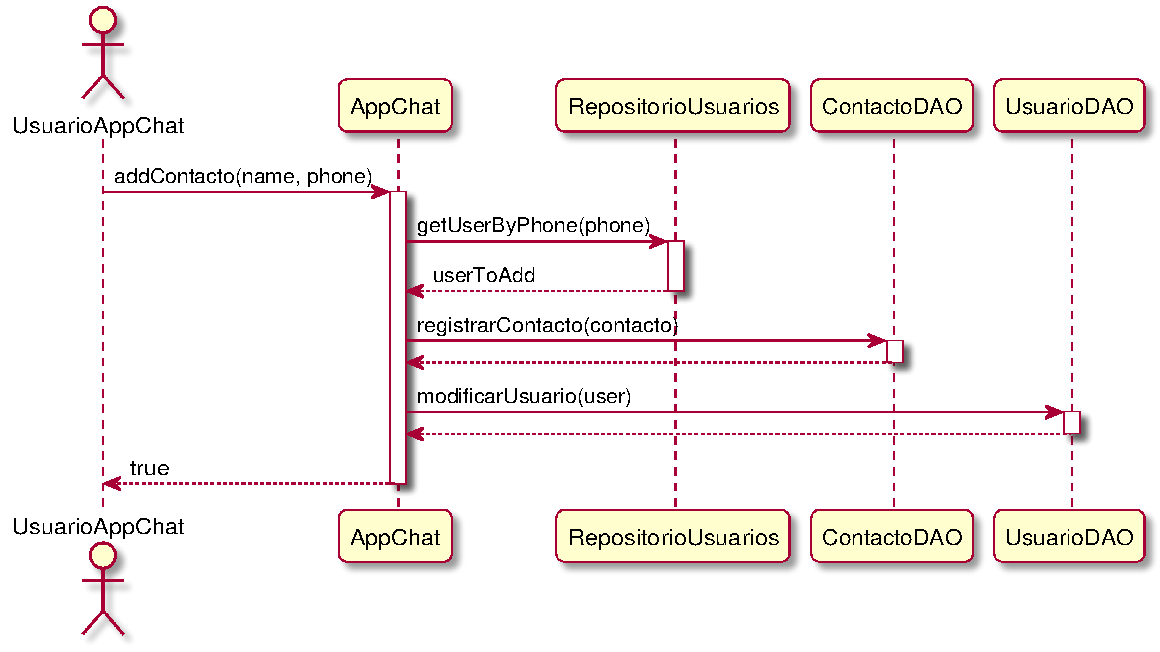
\includegraphics[width=0.86\linewidth]{figures/facade}
	\caption{Ejemplo simplificado de \textit{Facade} en el controlador de AppChat}
	\label{fig:facade}
\end{figure}

\clearpage

\subsection{Patrones de comportamiento}

\subsubsection*{Strategy}

Implementamos patrón de diseño \textit{Strategy} o Estrategia para diseñar los descuentos en AppChat. Nos permite definir una familia de algoritmos y encapsular cada uno de ellos. En el futuro, se puede implementar un nuevo descuento de forma sencilla, usando la interfaz definida.

\begin{figure}[H]
	\centering
	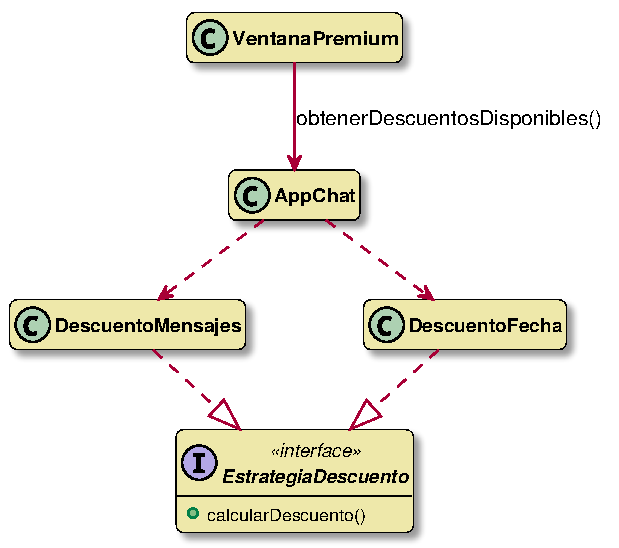
\includegraphics[width=0.4\linewidth]{figures/strategy_model}
	\caption{Modelo del patrón \textit{Strategy} para descuentos en Apphat}
	\label{fig:strategy}
\end{figure}

\subsection{Otros patrones de diseño}

\subsubsection{Data Access Object}

El patrón Data Access Object o DAO nos permite separar por completo la lógica de negocio de la lógica para acceder a los datos. De esta forma, las clases DAO proporcionarán los métodos necesarios para las operaciones de persistencia de los objetos, como guardar, borrar, editar o recuperar entidades. este patrón se usa junto factoría abstracta y adaptador para proporcionar una interfaz clara y desacoplar los paquetes.

\begin{figure}[H]
	\centering
	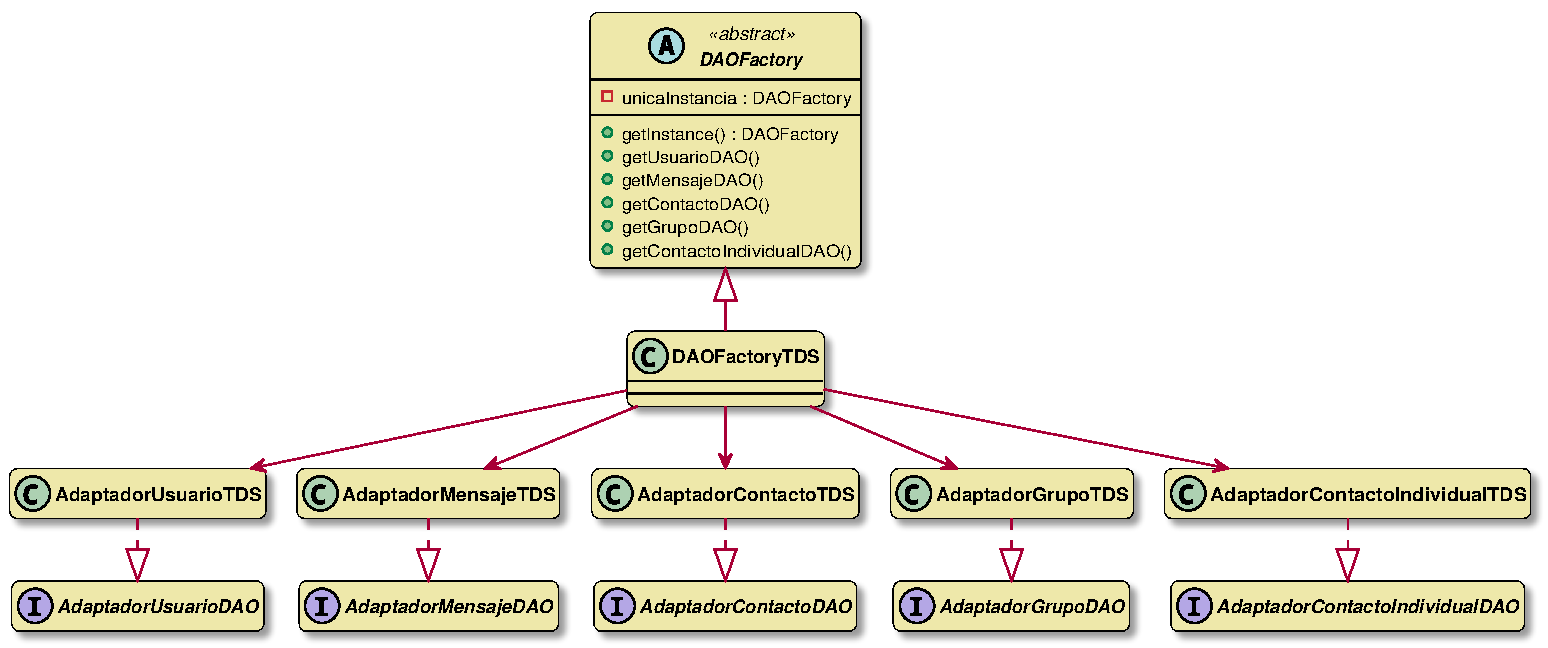
\includegraphics[width=1\linewidth]{figures/abstract_factory.pdf}
	\caption{Modelo del patrón DAO junto con \textit{Abstract Factory} y \textit{Adapter} de AppChat}
	\label{fig:absfactory}
\end{figure}


\subsubsection{Patrones usandos indirectamente}

En el desarrollo de AppChat, se han usado numerosas clases que implementan patrones de diseño en su código. Destacan algunos como:

\begin{itemize}
    \item \textbf{\textit{Singleton}, \textit{Facade}, y \textit{Abstract Factory}}: la librería DriverPersistencia proporcionada por los profesores usa proporciona una interfaz clara y un método de acceso global a la clase \texttt{FactoriaServicioPersistencia}.
    \item \textbf{\textit{Composite}}: las clases \texttt{JPanel}, \texttt{JFrame} y \texttt{Container} de Java AWT y Swing implementan este patrón para poder tratar objetos individuales y grupos de objetos de manera uniforme.
    \item \textbf{\textit{Observer}}: cuando usamos, por ejemplo, ``\textit{action listeners}'' en los botones de las ventanas.
    \item \textbf{\textit{Iterator}}: en las colleciones.
\end{itemize}

\clearpage

\section{Manual de usuario de AppChat}

\subsection{Inicio de sesión}

\begin{figure}[H]
	\centering
	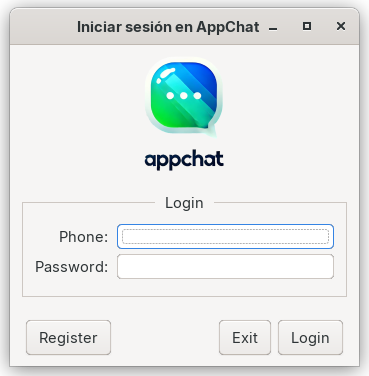
\includegraphics[width=0.4\linewidth]{figures/login}
	\caption{Inicio de sesión en AppChat}
	\label{fig:login}
\end{figure}

\subsubsection{Validación del inicio de sesión}

La interfaz gráfica ejecuta métodos y se comunica con el controlador para verificar el inicio de sesión. Si un usuario introduce un número no registrado o una contraseña incorrecta, el sistema mostrará un diálogo de error:

\begin{figure}[H]
	\centering
	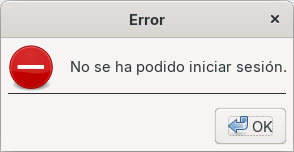
\includegraphics[width=0.4\linewidth]{figures/error-login.png}
	\caption{Error en el inicio de sesión}
	\label{fig:error-login}
\end{figure}

\subsection{Registro}

\begin{figure}[H]
	\centering
	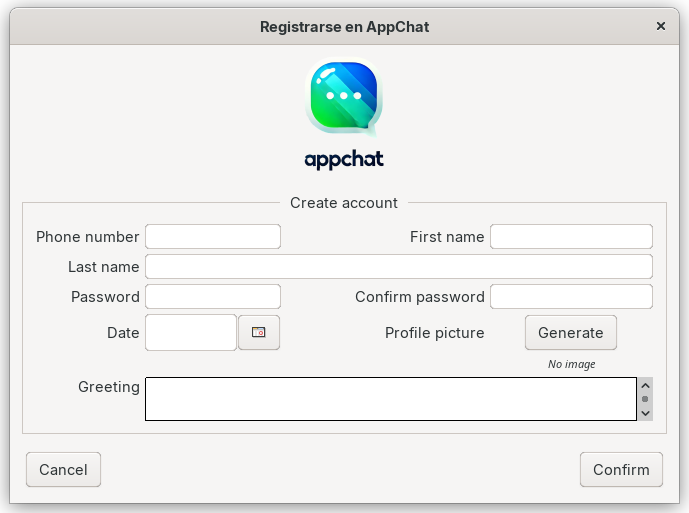
\includegraphics[width=0.6\linewidth]{figures/register}
	\caption{Registro en AppChat}
	\label{fig:register}
\end{figure}

\subsubsection{Validación de campos en el registro}

La interfaz gráfica también incorpora métodos para validar los campos antes de registrar a un usuario. Por ejemplo, si se intenta usar un número de teléfono ya registrado, el sistema mostrará un error al intentar crear la cuenta.

\begin{figure}[H]
	\centering
	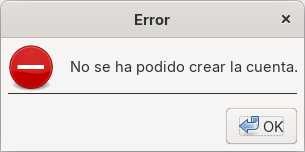
\includegraphics[width=0.35\linewidth]{figures/error-register}
	\caption{Error en el registro}
	\label{fig:error-register}
\end{figure}

Asimismo, si el usuario no introduce la misma contraseña los campos ``\textit{Contraseña}'' y ``\textit{Confirmar contraseña}'':

\begin{figure}[H]
	\centering
	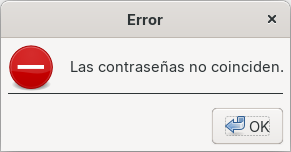
\includegraphics[width=0.35\linewidth]{figures/error-register-passwords}
	\caption{Error en el registro}
	\label{fig:error-register-passwords}
\end{figure}

\subsection{Vista principal}

\begin{figure}[H]
	\centering
	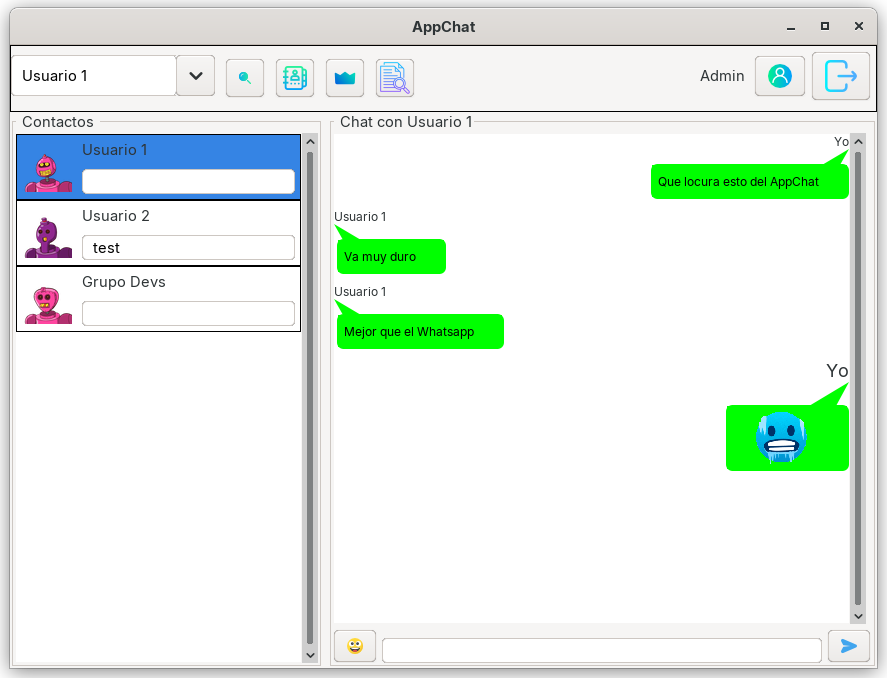
\includegraphics[width=0.75\linewidth]{figures/main}
	\caption{Ventana principal de AppChat}
	\label{fig:main}
\end{figure}

\subsubsection{Búsqueda de mensajes}

\begin{figure}[H]
	\centering
	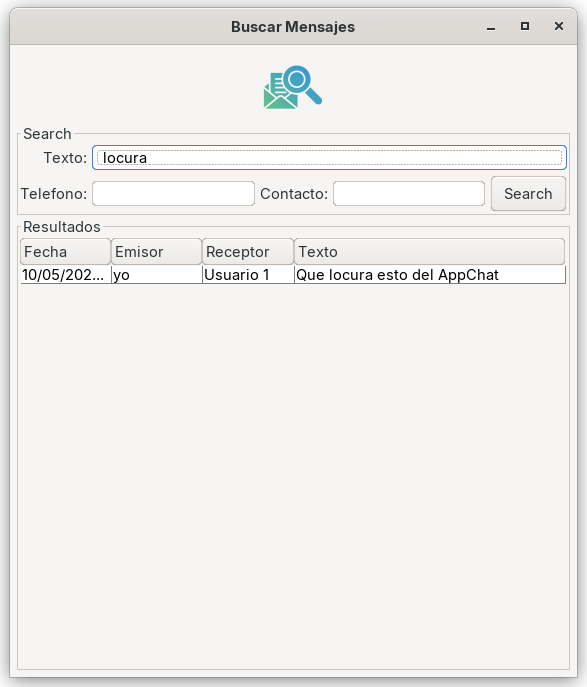
\includegraphics[width=0.5\linewidth]{figures/search}
	\caption{Búsqueda y filtrado de mensajes en AppChat}
	\label{fig:search}
\end{figure}

\subsection{Gestión de contactos}

\begin{figure}[H]
	\centering
	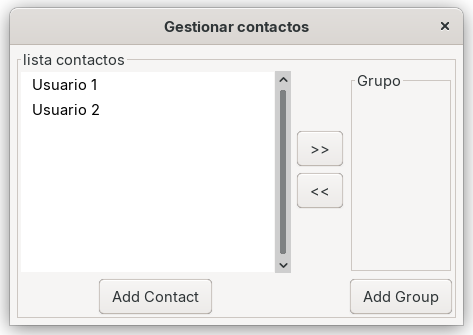
\includegraphics[width=0.4\linewidth]{figures/manage-contacts}
	\caption{Gestión de contactos de AppChat}
	\label{fig:manage-contacts}
\end{figure}

\subsubsection{Crear contacto}

\begin{figure}[H]
	\centering
	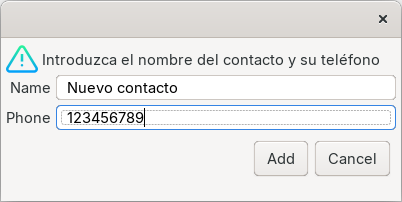
\includegraphics[width=0.5\linewidth]{figures/add-contact}
	\caption{Ventana para añadir contactos}
	\label{fig:add-contact}
\end{figure}

\textbf{Error al crear contacto}

\begin{figure}[H]
	\centering
	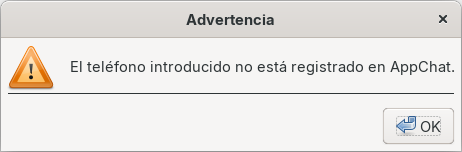
\includegraphics[width=0.4\linewidth]{figures/error-add-contact}
	\caption{Error al crear contacto}
	\label{fig:error-add-contact}
\end{figure}

\subsection{Perfil}

\begin{figure}[H]
	\centering
	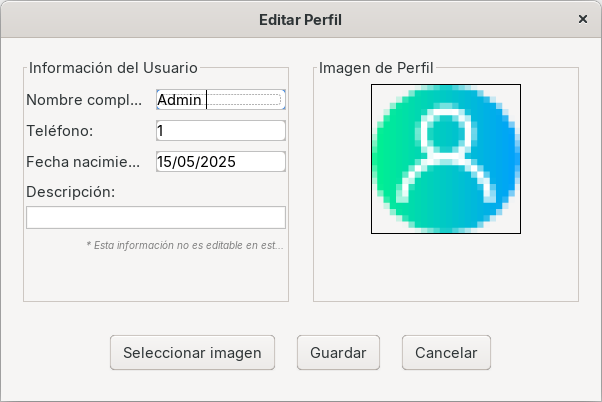
\includegraphics[width=0.65\linewidth]{figures/profile}
	\caption{Perfil de AppChat}
	\label{fig:profile}
\end{figure}

\subsection{Premium}

\begin{figure}[H]
	\centering
	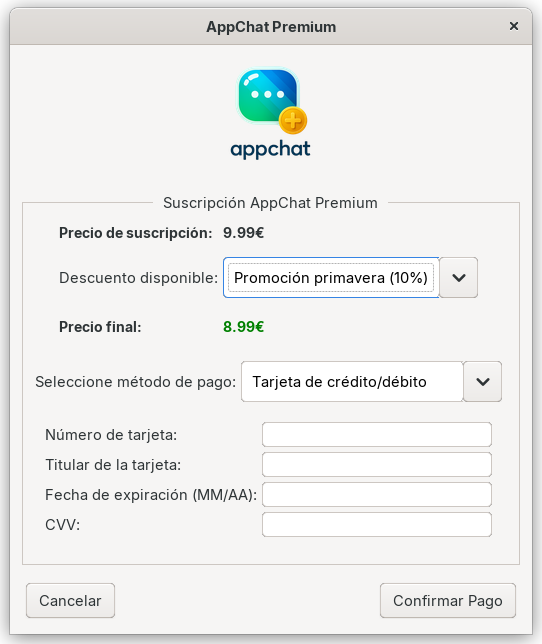
\includegraphics[width=0.35\linewidth]{figures/premium}
	\caption{Actualización a AppChat \textit{premium}}
	\label{fig:premium}
\end{figure}

\subsubsection{Confirmación del pago}

\begin{figure}[H]
	\centering
	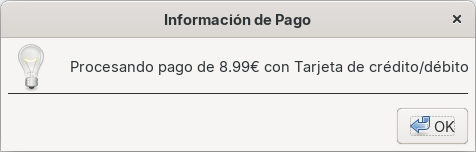
\includegraphics[width=0.35\linewidth]{figures/premium-payment}
	\caption{Confirmación del pago de AppChat \textit{premium}}
	\label{fig:premium-payment}
\end{figure}

\subsection{Exportación de mensajes en formato PDF}

Para este funcionalidad, se ha implementado también la posibilidad de poder exportar los mensajes con todos los contactos.

\begin{figure}[H]
	\centering
	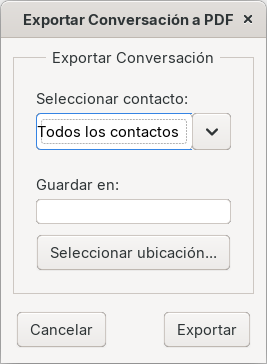
\includegraphics[width=0.25\linewidth]{figures/export}
	\caption{Ventana para exportar chats a formato PDF}
	\label{fig:export}
\end{figure}

\subsubsection{Ejemplo de documento generado tras exportar chats}

\begin{figure}[H]
	\centering
	\fbox{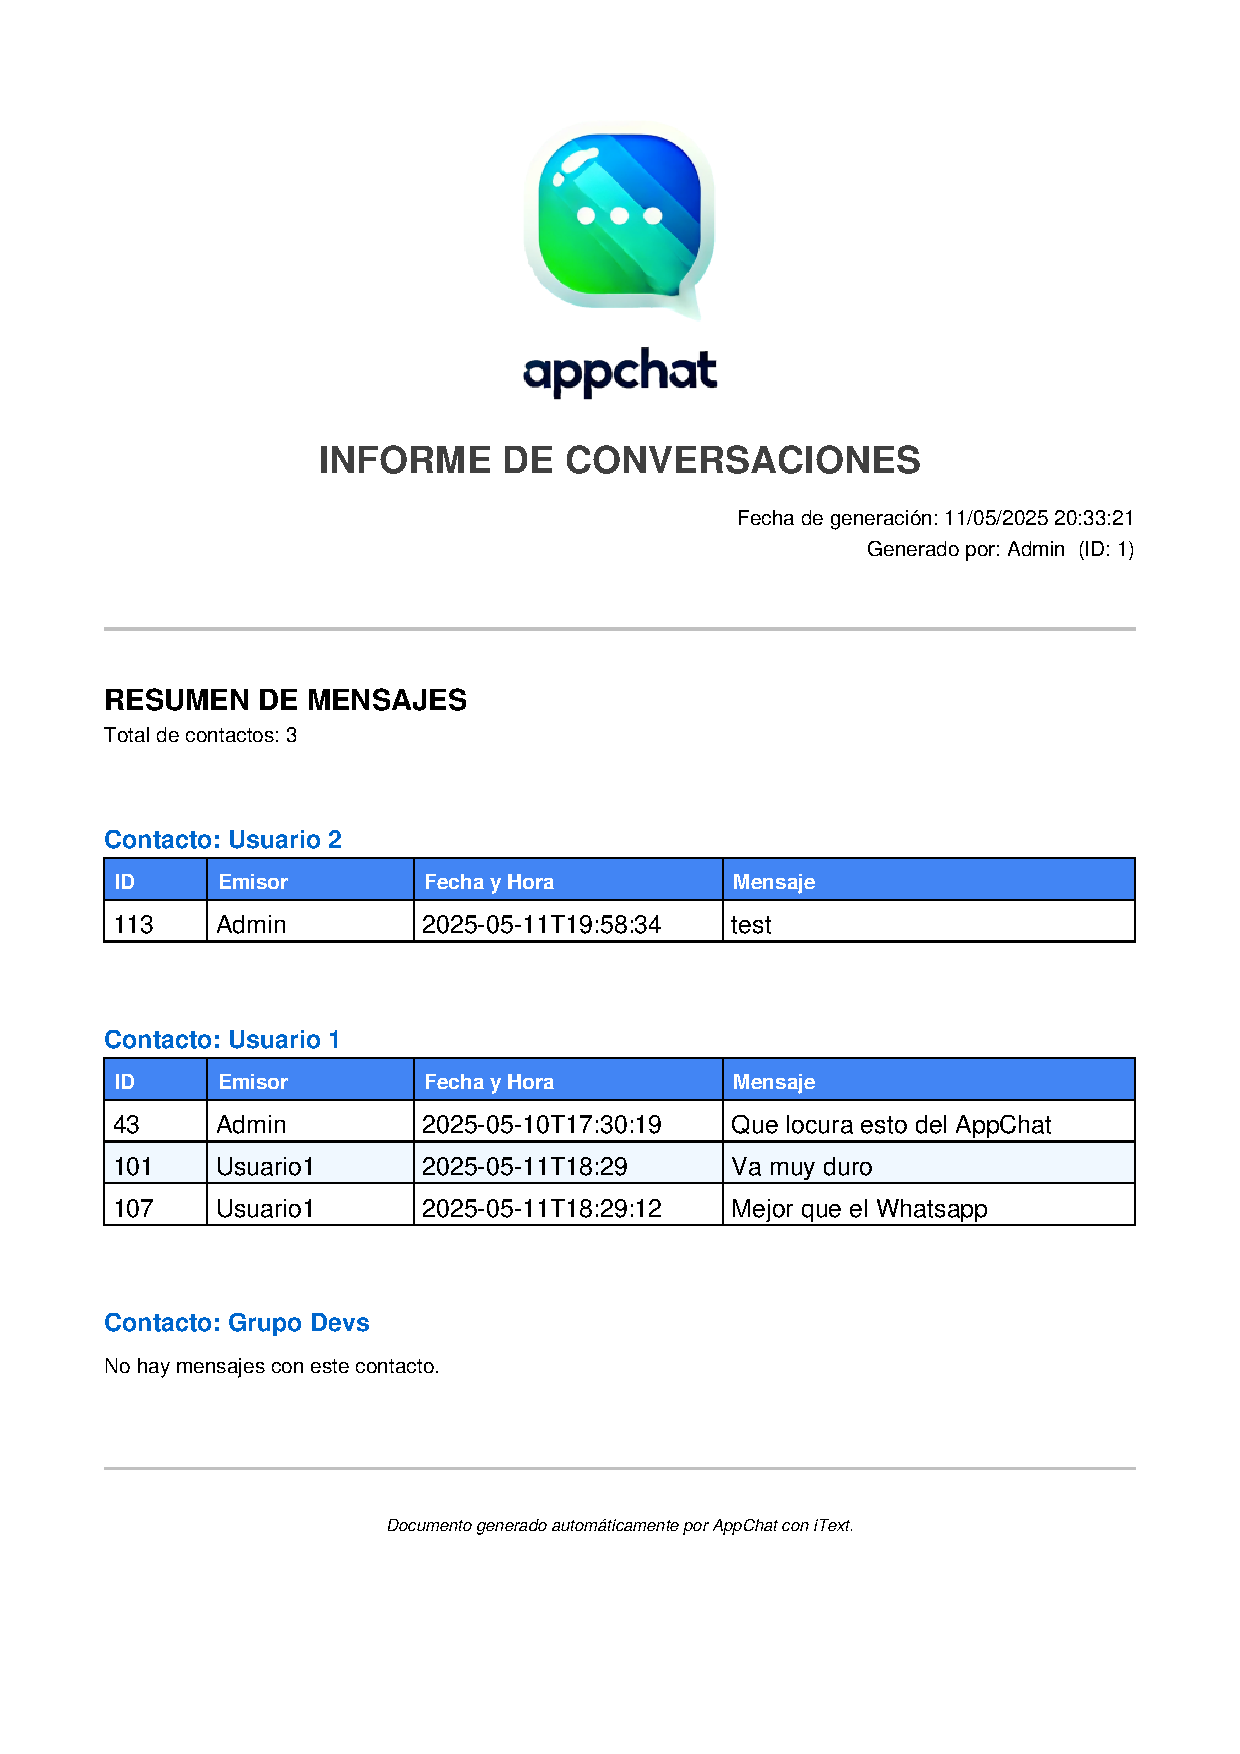
\includegraphics[width=0.7\linewidth]{figures/chat_exportado}}
	\caption{Confirmación del pago de AppChat \textit{premium}}
	\label{fig:chat-exportadot}
\end{figure}

\clearpage

\section{Conclusiones personales y distribución del trabajo}

Este proyecto ha sido el más extenso hasta el momento del grado en Ingeniería Informática también el primero en el que hemos desarrollado una aplicación gráfica de escritorio.\\

Ha sentado las bases sobre conceptos como la lógica de negocio (\textit{backend}) y la interfaz de usuario (\textit{frontend}). La interfaz proporcionada para la persistencia de datos también ha ayudado a comprender cómo se almacenan los objetos Java de forma persistence, y ha servido como una guía para más adelante usar JPA o Jakarta.\\

Al ser el primer proyecto de esta índole, las prioridades y ejecución del proyecto eran desconocidas. Si intentamos relacionar la práctica con otras asignaturas del grado, encontramos una gran similitud Gestión de Proyectos de Desarrollo de Software o Procesos de Desarrollo de Software. Hemos ejecutado el desarrollo de un proyecto de software y hemos aprendido la importancia del análisis de requisitos y del diseño de modelos.\\

Usar librerías externas nos ha mostrado la relevancia que tienen los patrones de diseño en el desarrollo de aplicaciones en la actualidad. Cada uno tiene un objetivo, y su uso resulta imprescindible en proyectos extensos.

\vspace{2ex}

\begin{table}[h!]
	\centering
	\begin{tabular}{|c|c|c|}
		\hline
		\textbf{Actividad} & \textbf{José Salinas} & \textbf{Hugo Sánchez} \\
		\hline
		\textit{Historias de usuario} & 4 h & 3 h \\
		\hline
		\textit{Diseño del modelo} & 4 h & 2 h\\
		\hline
		\textit{Implementación de la lógica} & 65 h & 90 h\\
		\hline
		\textit{Diseño de la interfaz gráfica} & 90 h & 65 h\\
		\hline
        \textit{Revisión y corrección de errores} & 20 h & 15 h\\
		\hline
        \textit{Mantenimiento del repositorio} & 2 h & 2 h\\
		\hline
		\textit{Documentación} &  4 h &  9 h \\
		\hline
		\textbf{Total} & 189 horas & 186 horas\\
		\hline
	\end{tabular}
	\caption{Distribución de horas entre los miembros}
\end{table}

\bibliographystyle{unsrt}
\bibliography{bibliography}


\end{document}